\chapter{Related work}
\label{chap:related_work}
In this chapter, the most relevant studies on the classification of music-elicited emotions have been reviewed. In 2013 T. Eerola and J. Vuoskoski \cite{eerola_review_2013} reviewed and categorized 251 studies related to music and emotions in terms of approaches, emotion models and stimuli. However, most of them are not comparable in terms of methods with the current study and the list is not updated with the most recent findings in the field of \ac{ER}. Therefore, the selection of studies reported below features some very well-known foundational ones that provide the theoretical framework to approach the selection of relevant features and the analysis of emotions using physiological signals, and some more recent ones focused on the classification of music-elicited emotions using machine learning algorithms. They have been ordered chronologically to emphasize the methodological progresses and their contribution to the design of the current experimental protocol and classification methods has been highlighted where appropriate. However, to underline the novelty of this research, only one reviewed study features the use of a wearable \ac{EEG} headset with 8 dry electrodes and another one artificially simulates the use of wearable device by picking 2 frontal electrodes from a bigger dataset recorded with 32 wet electrodes.

\section{Classification of music-elicited emotions}
\label{sec:classification_emotions}
L.A. Schmidt and L.J. Trainor \cite{schmidt_frontal_2001} were the first investigators that reviewed all the existing regional brain activation/emotion models and tried to systematically verify their validity for the analysis of music-elicited emotions. To do so, they designed an experiment selecting 4 orchestral excerpts that were pre-rated to represent the following classes:
\begin{enumerate}
\item Intense-unpleasant emotion: fear
\item Intense-pleasant emotion: joy
\item Calm-pleasant emotion: happy
\item Calm-unpleasant emotion: sad
\end{enumerate}
They hypothesized that:

\begin{itemize}
\item “Asymmetric frontal activation reflects emotional valence”
\begin{itemize}
\item Greater relative left frontal EEG activity for joy and happy musical pieces
\item Greater relative right frontal EEG activity for fear and sad musical pieces
\end{itemize}
\item “Regional brain activation reflects emotional intensity”
\begin{itemize}
\item A significant main effect for the intensity of affective musical excerpts on overall frontal EEG activity is characterized by a frontal pattern that would distinguish across valence as predicted by Davidson, Schmidt, and Dawson.
\item Right parietal activity would distinguish the intensity of the affective musical excerpts across valence as predicted by Heller.
\end{itemize}
\end{itemize}
Then, they recruited 59 participants (30 females) right-handed undergraduates of psychology between 18 and 34. Their EEG signal was recorded continuously for 60 seconds for each musical excerpt. The data was pre-processed and cleaned from artefacts, then analysed using \ac{DFT} with a Hanning window of 1-second width and 50\% overlap. 

\begin{figure}[h!]
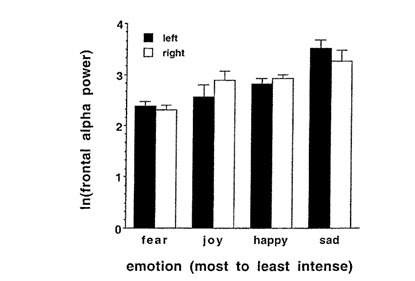
\includegraphics[width=10cm]{img/related_work/valence_hemisphere.png}
\centering
\caption{Valence by hemisphere interaction showed differences among the four musical excerpts on the left and right frontal EEG alpha power. Taken from \cite{schmidt_frontal_2001}}\label{fig_schmidt_valence_emo}
\end{figure}
Frequency-band specific power in the alpha band (8-13Hz) was derived from the \ac{DFT} output over the complete power spectrum. ANOVA analysis on Valence by Hemisphere interaction revealed a consistent behaviour between the left frontal EEG activity with positive valence songs and between the right frontal \ac{EEG} activity with negative valence songs (Fig. \ref{fig_schmidt_valence_emo}).
According to their findings, they could confirm that asymmetrical frontal activation indeed distinguished the valence of musical emotion: subjects exhibited greater relative left frontal EEG activity for musical excerpts with positive valence and vice versa on the right side for musical excerpts with negative valence (Fig. \ref{fig_schmidt_valence_alpha}), confirming their first hypothesis. Furthermore, the results showed that musically induced emotions elicit the same frontal brain regions as emotions induced through other means, which validates musical stimuli as good emotional elicitors for agnostic emotion classification. Intensity by hemisphere analysis reported main effects on intensity, but without interaction: subjects showed significantly greater activity in the frontal region as the affective stimuli became more intense. 

\begin{figure}[h!]
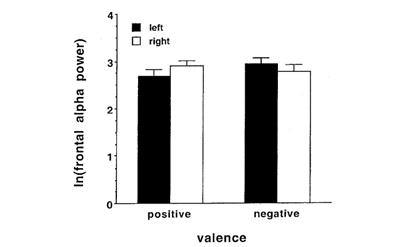
\includegraphics[width=10cm]{img/related_work/valence_hemisphere_alpha.png}
\centering
\caption{Valence by hemisphere interaction.Alpha power is inversely related to activity, positive left is accordingly lower for positive emotions and negative right is lower for negative emotion. Taken from \cite{schmidt_frontal_2001}}\label{fig_schmidt_valence_alpha}
\end{figure}
The frontal \ac{EEG} activity decreased from the presentation of the fear to the joy to the happy to the sad excerpts and it is consistent with the behavioural rating of intensity. Since they only used auditory stimuli, the lack of parietal differences might be due to the lack of external focus from environmental stimuli. 

\begin{figure}[h!]
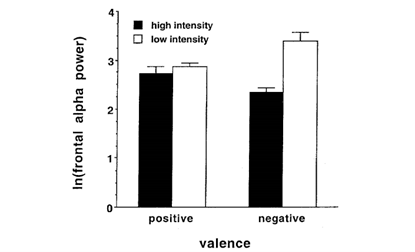
\includegraphics[width=10cm]{img/related_work/valence_intensity.png}
\centering
\caption{Valence by intensity interaction. Greater power (lower activity) in the low-intensity excerpts than in higher intensity excerpts, with a more extreme difference for negative valenced excerpts. Taken from \cite{schmidt_frontal_2001}}\label{fig_schmidt_valence_intensity}
\end{figure}
Valence by Intensity analysis showed that musical excerpts with higher intensity and positive valence elicited significantly higher activity compared with the opposite combination, low intensity and negative valence (Fig. \ref{fig_schmidt_valence_intensity}). This study is relevant for the analysis of music-elicited emotions because it provides a validation for the models proposed by Davidson, Fox and Heller that state the approach-withdrawal tendencies in the frontal \ac{EEG} activity: positive emotions are processed in the left anterior region of the brain, negative emotions are processed in the right anterior region of the brain. Regarding the intensity, or arousal dimension, of the emotions, the results are consistent with the models by Davidson, Dawson and Schmidt that correlate absolute frontal activation with the intensity of the emotional experience. However, in contrast with Heller’s model, they did not find relevant differences in the right parietal activity, possibly because of their experimental setup.
